% vim:ft=tex:
%
\documentclass[luatex]{beamer}

\setbeamercolor{background canvas}{bg=white}
\setbeamercolor{normal text}{fg=black!90}
\setbeamerfont{text}{size*={14}{1.4em}}

\setbeamertemplate{frametitle}{%
	\begin{centering}%
		\bigskip\Huge\insertframetitle\par\smallskip%
	\end{centering}%
}
\setbeamertemplate{navigation symbols}{}
\setbeamertemplate{footline}[text line]{}

\usepackage[english]{babel}
\usepackage{booktabs}
\usepackage{calc}
\usepackage{tikz}
\usetikzlibrary{arrows,shapes,fit,shadows,positioning,chains,%
	decorations.pathreplacing,decorations.pathmorphing,calc,%
	matrix}
\usepackage{pgfplots}

\definecolor{grey}{rgb}{0.5, 0.5, 0.5}
\definecolor{lightgrey}{rgb}{0.95, 0.95, 0.95}
\definecolor{grassgreen}{rgb}{0.1, 0.85, 0.2}
\definecolor{fadedbrown}{rgb}{0.85, 0.1, 0.1}
\definecolor{darkmagenta}{rgb}{0.65, 0.0, 0.65}
\definecolor{lightblue}{rgb}{0.5, 0.75, 1.0}
\definecolor{linkboxcolor}{rgb}{0.8, 0.8, 0.85}

% Minted
\usepackage{minted}
\setminted{
  autogobble   = true,
  breaklines   = true,
  codetagify   = true,
  encoding     = utf-8,
  outencoding  = utf-8,
  frame        = leftline,
  framerule    = 5pt,
  framesep     = 0.65em,
  xleftmargin  = 1em,
  xrightmargin = 1em,
  rulecolor    = \color{lightgrey},
}
\newmintinline[Mc]{c}{}
\newminted{c}{
  fontsize = \small,
  baselinestretch = 1.0,
}
\newmintinline[Mlua]{lua}{}
\newminted{lua}{
  fontsize = \small,
  baselinestretch = 1.0,
}

% Fonts
\usepackage[OT1]{fontenc}
\usepackage{fontspec}
\defaultfontfeatures{Ligatures=TeX}

\setmainfont{Andada}[
  Path           = fonts/,
  Extension      = .ttf,
  UprightFont    = *-Regular,
  ItalicFont     = *-Italic,
  BoldFont       = *-Bold,
  BoldItalicFont = *-BoldItalic,
  SmallCapsFont  = *SC-Regular,
]

\newfontfamily\RlwLight{Raleway}[
  Path           = fonts/,
  Extension      = .ttf,
  UprightFont    = *-ExtraLight,
  ItalicFont     = *-ExtraLight-Italic,
  BoldFont       = *-Light,
  BoldItalicFont = *-Light-Italic,
]

\setsansfont{Raleway}[
  Path           = fonts/,
  Extension      = .ttf,
  UprightFont    = *-Regular,
  ItalicFont     = *-Regular-Italic,
  BoldFont       = *-Bold,
  BoldItalicFont = *-Bold-Italic,
]

\setmonofont{InputMonoNarrow}[
  Scale          = MatchLowercase,
  Path           = fonts/,
  Extension      = .ttf,
  UprightFont    = *-Light,
  ItalicFont     = *-LightItalic,
  BoldFont       = *-Regular,
  BoldItalicFont = *-Italic,
]

\newfontfamily\SymbolaFont{Symbola}[
	Path          = fonts/,
	Extension     = .ttf,
]
\newcommand\Symbol[1]{{\SymbolaFont#1}}

% Symbols
\newcommand\LeafOpen{\Symbol{🙠}}
\newcommand\LeafClose{\Symbol{🙣}}

\title{\textsc{Eöl}}
\subtitle{Automatic bridging of native code to Lua using existing debugging information}
\author{Adrián Pérez de Castro}
\institute[UDC]{
	
\begin{tikzpicture}[y=0.80pt, x=0.8pt,yscale=-1, inner sep=0pt, outer sep=0pt, scale=0.2]
	  \path[fill=magenta,nonzero rule] (220.7188,106.4062) -- (382.3633,33.4609) ..
		controls (341.6836,12.8594) and (284.3281,-0.0039) .. (220.7227,-0.0039) ..
		controls (157.1016,-0.0039) and (99.7461,12.8594) .. (59.0742,33.4609) --
		(220.7188,106.4062);
	  \path[fill=magenta,nonzero rule] (440.9648,89.9531) .. controls
		(436.4648,76.9375) and (427.1289,64.7109) .. (413.8828,53.7188) --
		(233.1914,105.5312) -- (440.9648,89.9531);
		\path[fill=magenta,nonzero rule] (414.9375,161.0898) .. controls
		  (428.0547,149.9570) and (437.2305,137.6055) .. (441.4414,124.4531) --
		  (232.9805,109.8984) -- (414.9375,161.0898);
		\path[fill=magenta,nonzero rule] (220.7305,109.2188) -- (57.9609,181.6680) ..
		  controls (98.6992,202.6055) and (156.5195,215.6992) .. (220.7227,215.6992) ..
		  controls (284.9102,215.6992) and (342.7344,202.6055) .. (383.4805,181.6680) --
		  (220.7305,109.2188);
	  \path[fill=magenta,nonzero rule] (0.0000,124.4531) .. controls (4.2109,137.6055)
		and (13.3867,149.9570) .. (26.4961,161.0898) -- (208.4492,109.8984) --
		(0.0000,124.4531);
	  \path[fill=magenta,nonzero rule] (208.2422,105.5312) -- (27.5625,53.7109) ..
		controls (14.3164,64.7070) and (4.9766,76.9336) .. (0.4727,89.9531) --
		(208.2422,105.5312);
	\end{tikzpicture}
	\vspace{0.5em}

	Universidade da Coruña}
\date[Sep 2015]{September, 2015}

\begin{document}

\setbeamertemplate{background canvas}{%
	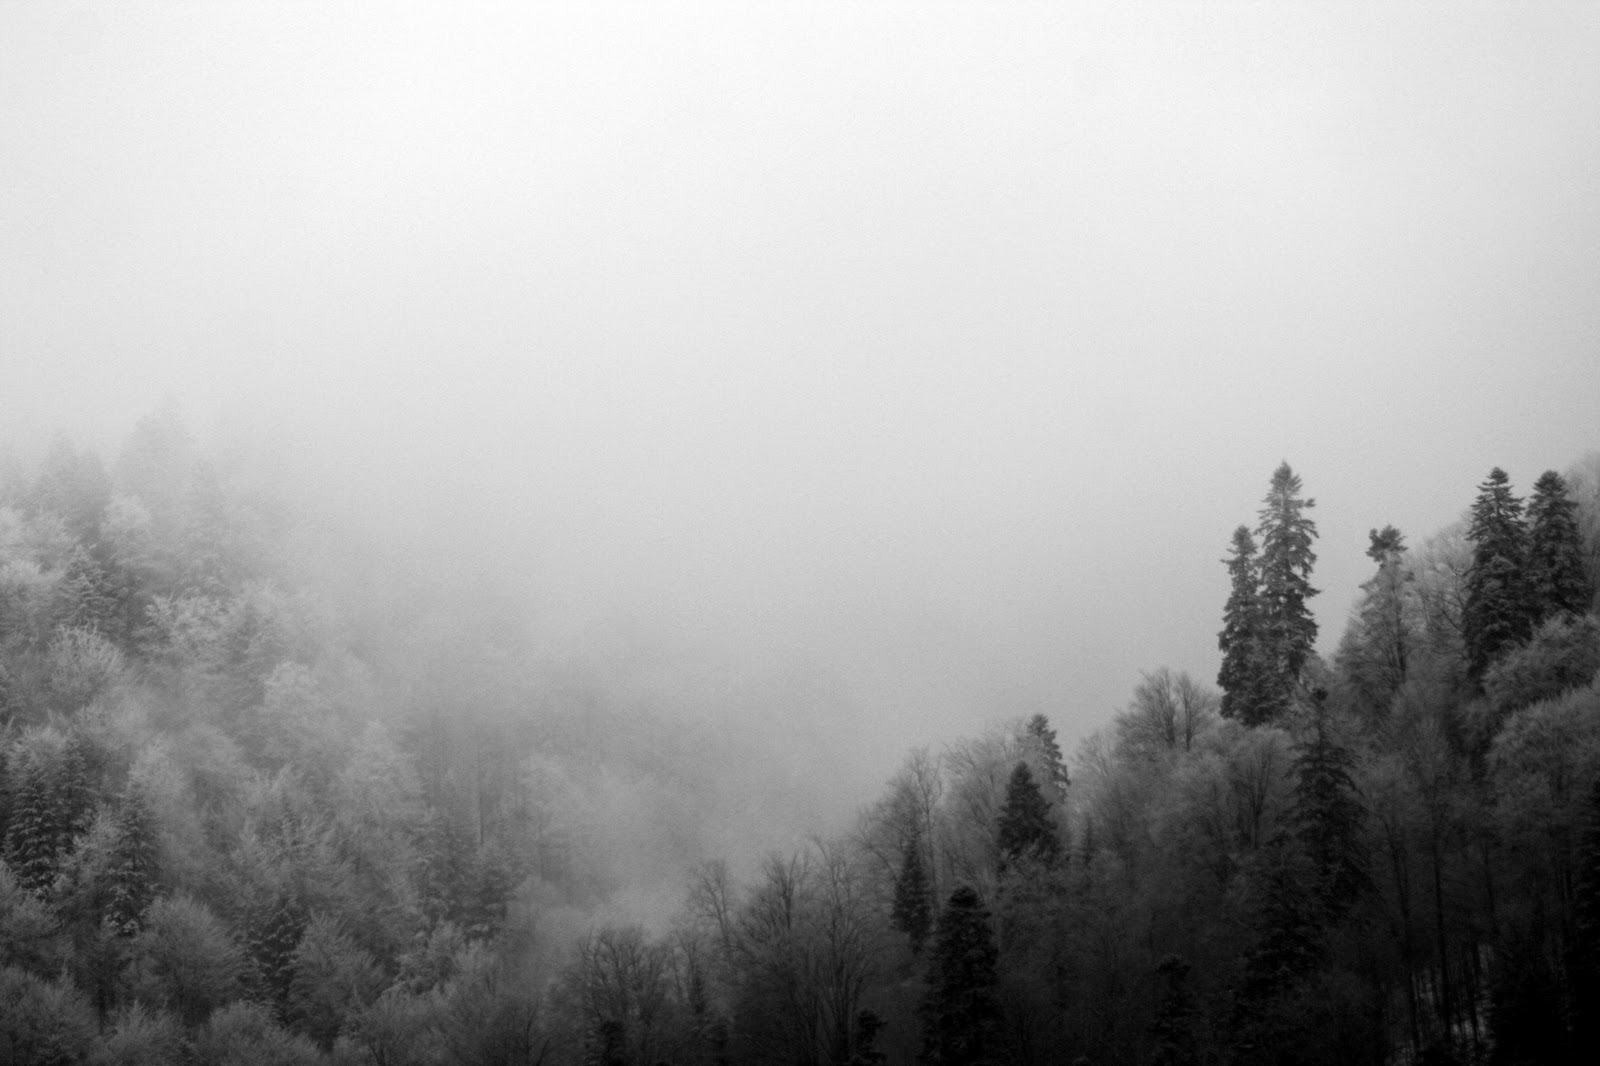
\includegraphics[height=\paperheight]{img/forest.jpg}}
% \setbeamercolor{title}{fg=black}
% \setbeamercolor{block body}{fg=white}

\maketitle

\setbeamertemplate{background canvas}{}
% \setbeamercolor{normal text}{fg=black!90}

\begin{frame}{Outline}
	\tableofcontents
\end{frame}


\section{Lua}

\subsection{Quick Introduction}

\begin{frame}

	\centering
	
\includegraphics[height=0.15\textheight]{img/lua-logo.pdf}
	\vspace{3em}
	\begin{quote}
		Lua is apowerful, fast, lightweight, embeddable
		scripting language.
	\begin{flushright}
		\begin{scriptsize}
		— \url{http://www.lua.org/about.html}
		\end{scriptsize}
	\end{flushright}
	\end{quote}
	\vfill

	\begin{itemize}
		\item Single data structure \visible<2->{$\rightarrow$ \emph{tables}}
		\item Extensible semantics \visible<3->{$\rightarrow$ \emph{metatables}}
		\item Automatic memory management \visible<4->{$\rightarrow$ \emph{GC}}
		\item Bytecode, register-based VM
	\end{itemize}

	\note[itemize]{
		\item Intially created as a data description language at Tecgraf
			PUC-Rio, for in-house software development: trade barriers were in
			effect for software and computer hardware.
		\item Petrobras was one of the first users of SOL and DEL, the
			predecessors of Lua.
		\item Tables can be used as hash tables, arrays, and objects.
			Particularly well suited for data description.
		\item Influences by Module (control structures), AWK (tables), and
			LISP (everything is a list\^W table)
		\item Widely used in the games industry (WoW).
	}
\end{frame}


\begin{frame}[fragile]{Lua by Example}
  \begin{luacode}
    animal = {
      name = "Unnamed",
      kind = "living creature",
      describe = function (self)
        print(self.name .. " is a " .. self.kind)
      end,
    }

    f = setmetatable({ kind="cat", name="Fifi" },
                     { __index=animal })
    t = setmetatable({ name="Tom", },
                     { __index=animal })
    f:describe()  --> Fifi is a cat
    t:describe()  --> Tom is a living creature
  \end{luacode}

	\note[itemize]{
		\item First a base object (which is a table) is defined
		\item Functions are first-class values, and as such can
			be values in a table
		\item Metatables allow defining the runtime behaviour of
			certain operations. Here we set \texttt{\_\_index}
    		so the fields not found in \texttt{cat} or \texttt{dog}
    		are looked up in the \texttt{animal} table instead. This
    		effectively creates a prototype-style chain of obejcts.
	}
\end{frame}


\subsection{Accessing Native Code}


\begin{frame}[fragile]{Going Native: Try I}

Fact: Lua has a very minimal and small standard library.

\pause
\textbf{How is additional functionality provided?}

\pause
\vspace{2em}

\begin{luacode}
function isdir(path)
  local fd = io.popen("test -d " .. path)
  fd:read("*a") -- Discard output
  local ok, reason, code = fd:close()
  return ok and reason == "exit" and code == 0
end
\end{luacode}
\vspace{2em}

\pause
\hfill …but this is \emph{cheating}

\pause
\hfill …and horrible in many ways

\note[itemize]{
	\item Fatality 1: Spawning a child process just to check something that is
		provided as a system call.
	\item Fatality 2: The \texttt{path} variable needs to be quoted properly.
	\item Fatality 3: \texttt{io.popen} uses \texttt{system()}, which does
		shell expansion, and is a security hole.
	\item What we really want is to be able to call native functions.
}

\end{frame}


\begin{frame}{Going Native: Try II}

	Civilized ways:

	\begin{enumerate}
		\item Lua C API
		\item Wrappers over the C API
		\item Binding generators
		\item Foreign Function Interfaces
		\item \textsc{Eöl} (this project)
	\end{enumerate}

\end{frame}


\begin{frame}[fragile]{\texttt{isatty}}
\begin{luacode}
function isatty(fileno)
  -- ???
end
\end{luacode}
\end{frame}


\begin{frame}[fragile]{\texttt{isatty}: Lua C API}

C:

\begin{ccode}
static int f_isatty(lua_State *L) {
  lua_Integer fileno = luaL_checkinteger (L, 1);
  lua_pushboolean (L, isatty ((int) fileno));
  return 1;
}

int luaopen_isatty (lua_State *L) {
  lua_pushcfunction (L, f_isatty);
  return 1;
}
\end{ccode}

Lua:

\begin{luacode}
	local isatty = require("isatty")
	print(isatty(0), type(isttyatty(0)))
	-- Output: true boolean
\end{luacode}
\end{frame}


\begin{frame}{Binding Generators}
	\begin{itemize}
		\item Tools that create bindings in an automated way.
		\item<2-> They require an extra compilation step.
		\item<2-> Cleanup of the C definition may be needed.
	\end{itemize}

	\note[itemize]{
		\item Some Lua-specific binding generators exist, they are either
			outdated or are not very complete.
		\item SWIG is the standard to beat... but it's still a binding
			generator, requires an extra step, and so on.
	}
\end{frame}


\begin{frame}[fragile]{\texttt{isatty}: LuaJIT FFI}
\begin{luacode}
	local ffi = require("ffi")
	ffi.cdef("int isatty(int)")
	local isatty = ffi.C.isatty
	print(isatty(0), type(isatty(0)))
	-- Output: 1 number
\end{luacode}

\visible<2->{
	\begin{itemize}
		\item No need to manually write glue code
		\item Precise type information
	\end{itemize}
}

\end{frame}


\begin{frame}[fragile]{\texttt{isatty}: Ideal FFI}
\begin{luacode}
	local eol = require("eol")
	local isatty = eol.C.isatty
	print(isatty(0), type(isatty(0)))
	-- Output: 1 number
\end{luacode}

\hspace{4em}
\visible<2->{
	\begin{itemize}
		\item No need to manually write glue code
		\item Precise type information
		\item \textbf{No manual function declaration} (\Mlua|ffi.cdef|)
	\end{itemize}
}

\end{frame}


\begin{frame}{Ideal FFI = \textsc{Eöl}}
	\begin{quote}
		In order to implement the “ideal” FFI we need information
		about functions, their parameters, and involved data types.
	\end{quote}
	\pause
	\begin{itemize}
		\item The compiler already knows that information.
		\pause
		\item The compiler \emph{can} write it as debugging information.
	\end{itemize}
\end{frame}


\section{\textsc{Eöl}}

\pgfdeclarelayer{background}
\pgfdeclarelayer{foreground}
\pgfsetlayers{background,main,foreground}

\tikzstyle{bdBox} = [
	rectangle, drop shadow, draw=black, thick, fill=white,
	text centered, minimum height=2em, minimum width=3em,
]
\tikzstyle{bdProcBox} = [
	rounded corners, fill=blue!10, text centered
]
\tikzstyle{bdProcLine} = [
	draw, thick, color=blue!20
]
\tikzstyle{bdCircle} = [
	circle, fill=blue!20, draw=black,
]
\tikzstyle{bdLine} = [draw, thick]
\tikzstyle{bdArrow} = [bdLine, >=triangle 45, ->]


\tikzstyle{datablob} = [
  rectangle, rounded corners, drop shadow, draw=black, thick,
  text centered, minimum height=2em, minimum width=3em, fill=blue!20,
]
\tikzstyle{die}      = [start chain=going below, node distance=1mm]
\tikzstyle{dielabel} = [on chain]
\tikzstyle{dieitems} = [
  rectangle split, rectangle split parts=#1, rectangle split part align=left,
  thick, draw, fill=blue!10, on chain,
]
\tikzstyle{enumitems} = [
  rectangle split, rectangle split parts=#1, rectangle split part align=left,
  thick, rounded corners,
  color=black!50, fill=black!5, draw=black!50,
  minimum height=3em,
]
\tikzstyle{valuefrom} = [draw=black!50, thick, dashed]
\tikzstyle{arrow} = [draw, thick, >=triangle 45, ->]
\tikzstyle{datain} = [
  draw=black!80, thick, fill=blue!10, rectangle,
  text centered, minimum height=1.3em, text width=10em,
]
\tikzstyle{component} = [
  draw=black,
  thick,
  fill=green!10,
  rectangle,
  text centered,
  minimum height=2em,
  text width=6em,
  rounded corners,
  drop shadow,
]
\tikzstyle{uses} = [
  draw,
  very thick,
  >=triangle 45,
  ->,
  dashed,
]
\tikzstyle{contains} = [
  draw,
  thick,
  >=triangle 45,
  -*,
]


\begin{frame}{\textsc{Eöl}}
	\begin{center}
	\Huge
	FFI + DWARF/ELF
	\end{center}

	\pause

	\begin{center}
	Automatic binding system for the Lua programming language which allows
	seamless usage, at runtime, of libraries written in C.
	\end{center}
\end{frame}


\subsection{Architecture}

\begin{frame}{Design}

\resizebox{\textwidth}{!}{
\begin{tikzpicture}[node distance=2cm]
	\node[component] (library) {Library};
	\node[component] (typecache) [above of=library]   {Type Cache};
	\node[component] (ctype)     [right=1cm of library]   {CType};
	\node[component] (function)  [right=1cm of ctype]     {Function};
	\node[component] (variable)  [right=1cm of function]  {Variable};
	\node[component] (typeinfo)  [above of=function]  {Type Information};
	\node[datain]    (dwarf)     [above=1cm of typecache]
								  {DWARF debugging information};

	\node (luadata) [below right of=ctype] {Visible in Lua as userdata};
	\node (elf)     [above=0cm of dwarf]   {ELF shared object};

	\path[uses] (function) -- (typeinfo);
	\path[uses] (variable) -- (typeinfo);
	\path[uses] (ctype) -- (typeinfo);
	\path[uses] (typecache) -- (dwarf);
	\path[contains] (library) -- (typecache);
	\path[contains] (typecache) -- (typeinfo);

	\begin{pgfonlayer}{background}
	  \node[datablob] (elfbox) [fit=(dwarf) (elf), drop shadow] {};
	  \node[fill=yellow!20, rectangle, rounded corners] (wrappers)
	  [fit=(library) (variable) (function) (luadata)] { };
	\end{pgfonlayer}
\end{tikzpicture}
}

\end{frame}


\subsection{DWARF + ELF}

\begin{frame}{ELF}
\begin{columns}
\begin{column}{0.55\textwidth}
\resizebox{\textwidth}{!}{
\begin{tikzpicture}[node distance=1.5mm, bend angle=0]
	\node[bdBox] (elfheader) [minimum width=10em, start chain=going below, on chain] {ELF header};
	\node[bdBox] (prgheader) [minimum width=10em, on chain] {Program header};
	\node[bdBox] (sect-text) [minimum width=10em, on chain] {\texttt{.text}};
	\node[bdBox] (sect-rodata) [minimum width=10em, on chain] {\texttt{.rodata}};
	\node (ellipsis) [minimum width=10em, on chain] {...};
	% \node[bdBox] (sect-data) [minimum width=10em, on chain, yshift=-1em] {\textt{.data}};
	\node[bdBox] (sect-data) [minimum width=10em, on chain] {\texttt{.data}};
	\node[bdBox] (secthdrtable) [minimum width=10em, on chain] {Section header table};
	\draw[decorate, decoration={brace}] let \p1=(sect-text.north),
		\p2=(sect-rodata.south) in ($(2.2, \y1)$) -- ($(2.2, \y2)$)
		node[midway] (g1) {};
	\draw[decorate, decoration={brace}] let \p1=(ellipsis.north),
		\p2=(sect-data.south) in ($(2.2, \y1)$) -- ($(2.2, \y2)$)
		node[midway] (g2) {};
	\draw[->, bend right, >=latex, bend right, thick]
		(elfheader.east) to [out=90,in=90] (g1.east);
	\draw[->, bend right, >=latex, bend right, thick]
		(elfheader.east) to [out=90,in=90] (g2.east);
	\draw[->, bend left, >=latex, bend right, thick]
		(secthdrtable.west) to [out=90,in=90] (sect-text.west);
	\draw[->, bend left, >=latex, bend right, thick]
		(secthdrtable.west) to [out=90,in=90] (sect-rodata.west);
	\draw[->, bend left, >=latex, bend right, thick]
		(secthdrtable.west) to [out=90,in=90] (sect-data.west);
\end{tikzpicture}
}
\end{column}
% \begin{column}{0.1\textwidth}
% \end{column}
\begin{column}{0.45\textwidth}
	\begin{itemize}
		\item Headers
			\begin{itemize}
				\item Fixed part
				\item Variable tables
			\end{itemize}
		\item Segments
			\begin{itemize}
				\item Runtime
				\item Executable shape
			\end{itemize}
		\item Sections
			\begin{itemize}
				\item Offline
				\item Arbitrary data
			\end{itemize}
	\end{itemize}
\end{column}
\end{columns}
\end{frame}


\begin{frame}{DWARF}
\centering
\resizebox{0.75\textwidth}{!}{
\begin{tikzpicture}[die]
  \node[dielabel] (taglabel) {Tag};
  \node[dieitems=1] (tag) {\texttt{DW\_TAG\_pointer}};
  \node[dielabel] (attrlabel) {Attributes};
  \node[dieitems=1] (attributes) {\texttt{DW\_AT\_type}};
  \node[dielabel] (rtaglabel) [right=3cm of tag, yshift=-3.5mm] {Tag};
  \node[dieitems=1] (rtag) {\texttt{DW\_TAG\_pointer}};
  \node[dielabel] (rattrlabel) {Attributes};
  \node[dieitems=1] (rattributes) {\texttt{DW\_AT\_type}};
  \node[datablob] (basedie) [right=2cm of rattributes] {Type DIE};
  \path[arrow] (rattributes.text east) -- (basedie);
  \begin{pgfonlayer}{background}
    \node[datablob] (die) [fit=(taglabel) (attributes) (tag)] {};
    \node[datablob] (rdie) [fit=(rtaglabel) (rattributes) (rtag)] {};
  \end{pgfonlayer}
  \path[arrow] (attributes.text east) -- (rdie.west);
\end{tikzpicture}
}

	\vspace{2em}

	\begin{columns}
	\begin{column}{0.5\textwidth}
		ELF sections:
		\begin{itemize}
			\item \texttt{.debug\_types}
			\item \texttt{.debug\_info}
			\item \texttt{.debug\_}…
		\end{itemize}
	\end{column}
	\begin{column}{0.5\textwidth}
		DWARF information:
		\begin{itemize}
			\item Tree-like structure
			\item Nodes: DIEs \& TUEs
			\item Tagged attributes
		\end{itemize}
	\end{column}
	\end{columns}
\end{frame}


\section{Demos}

\begin{frame}
	\centering
	\Symbol{\Huge 🖮}
	\Large

	Demo Time!
\end{frame}


\setbeamertemplate{background canvas}{%
	
\includegraphics[height=\paperheight]{img/theend3.jpg}}
\begin{frame}
\end{frame}

\end{document}
